\chapter{Android Basics}\label{chapter:android_basics}

\section{Android Architecture}\label{section:android_architecture}
To provide copy protection mechanisms for Android apps,
of course a deep understanding of the Android system itself
is necessary. As mentioned in~\autoref{chapter:android_status_quo},
Android is built on the Linux kernel. Android does provide not
only shell binaries (Linux kernel) but also a GUI environment
as well as predefined frameworks and a complete environment
for developers to write apps in the Java programming language.
That's why Android is considered to be a ``full software stack''
~\parencite{levin}. Although it's built on Linux,
Google did modify the Linux kernel to their need.
As a result, the Android kernel differs
incompatibly with the Linux kernel since version 2.6.27.

The difference at kernel-level is not massive compared to
the differences at user-mode where Android does have entirely new
components, namely:

\begin{itemize}
\item Dalvik Runtime including the Dalvik Virtual Machine (DVM)
respectively the Android Runtime (ART) since Android version > 5.0.
\item The Bionic C-Library instead of the GNU C Library (GlibC)
\item Hardware Abstraction Layer (HAL)
\item Java Native Interface (JNI)
\item Android specific frameworks
\end{itemize}

\autoref{fig:androidvslinux} visually summarizes the difference
between Android and Linux.

\begin{figure}[htb]
  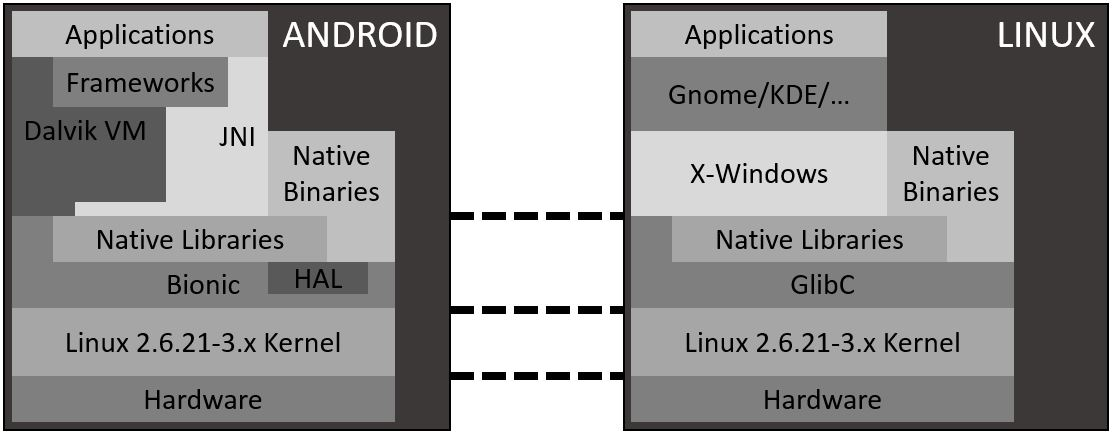
\includegraphics[width=\textwidth]{figures/androidvslinux}
  \caption[Android vs Linux]{Android and Linux comparison
  ~\parencite{levin}}
  \label{fig:androidvslinux}
\end{figure}

The Android specific frameworks are the core work that makes Android
special. They simplify the creation process of applications massively.
Developers can use the high level language Java rather than developing
in C/C++. Additionally, there is a rich set of APIs to solve most of
programmers everyday problems.

In order to get Java programs run on Android, the DVM is introduced
which is quite similar to a Java Virtual Machine (JVM).
The DVM provides an interface between the operating system and
the Java application world, after all the execution of Java programs.
The difference between DVM and JVM is the alternative form of bytecode
which gets executed in the VM. Another difference is that Dalvik is
register-based in contrast to JVM'S stack based architecture.
DVM is optimized for mobile devices
in terms of efficiency and sharing memory and is using the
Dalvik Executable format (DEX) as bytecode which is still device
independent ~\parencite{levin}. These \code{.dex} files are being
packed into Java libraries (JAR) or into Android Application Packages (APK).

With Android version 5.0, Google did introduce ART.
The prior Dalvik runtime does use Just-In-Time (JIT) compiling
where executable machine code is created not until runtime.
ART on the other hand does use Ahead-Of-Time (AOT) compilation
which compiles an app to machine code at installation time.
The reason for JIT in the first place were among other things
storage limitations of mobile devices at the time Android was released
~\parencite{levin}. As a result, the ART apps installation time
is increased as well as the required storage space as a tradeoff
to the app startup and runtime performance. As we will see,
Dalvik is still very much deep-seated in Android even under ART
and is impeding the development of a revolutionary copy protection
mechanism under ART.

The JNI provides an opportunity to write Java programs with embedded
native processor specific code to escape from the VM world
such as direct hardware access.
It is mostly used to optimize the performance for apps (e.g. games)
or to hinder reverse engineering of the application code.
Google does provide a Native Development Kit (NDK) to help
developers creating native libraries ~\parencite{ndk}.

Bionic is the Android corresponding GlibC library which was created
for license and simplicity reasons. Overall, it is more lightweight
than the GlibC and well adapted for Android.

Since Android is likely to run on a great variety of devices,
it has to support a big amount of different hardware versions.
The HAL addresses this problem and
standardizes the interface by allowing hardware vendors
to implement their own drivers ~\parencite{levin}.

\section{Android Apps}\label{section:android_apps}
Apps are the most abstract level of the Android software stack.
Generally there are either system-(mostly preinstalled) or user-apps.
The system apps storage location (\code{/system/apps/}) differs from
the user apps (\code{/data/apps/}). System apps are included into the
distributed OS whereas user-apps can be installed and updated
via the Android Debug Bridge (ADB), app stores
like the Google Play Store or directly on the device by opening
downloaded app files.

Every app has its own sandboxed environment. That means that
apps can not access data from other apps and they can only access
resources those permissions were granted during installation time.
These are one of the basic Android security concepts,
the Privilege separation and the principle of the least
privileges \parencite{securityinternals}.

Apps do have several components, the main ones are:

\begin{itemize}
\item Activities
\item Services
\item Content providers
\item Broadcast receivers
\end{itemize}

Activities do represent a screen view in the UI ready for user
interaction. They can be started independently even though one Activity
is chosen to be the one that starts when the user clicks on the
app icon. Services are purely functional and are not represented
at the UI compared to Activites. Their utilisation are mostly time
consuming operations in the background of an app like server
communication or computational tasks. Since apps are sandboxed,
they can't access each others data which is a huge limitation.
That's why Content providers do offer an interface to the app
data which is chosen to be exchanged.
They use a lower level Inter Process Communication (IPC) protocol
provided by the Android Stack.
With Broadcast receivers, an app can react on systemwide events
(broadcasts) \parencite{securityinternals}.

Apps are distributed in form of \code{.apk} files.
The APK file is a container for several files and is an extension to
JAR which is in turn an extension to the ZIP file format.
Thus the content of the APK can be extracted with standard ZIP
compression tools \parencite{securityinternals}.

\autoref{fig:apk_content} lists the content of an APK container
after extraction.

\begin{figure}[htb]
  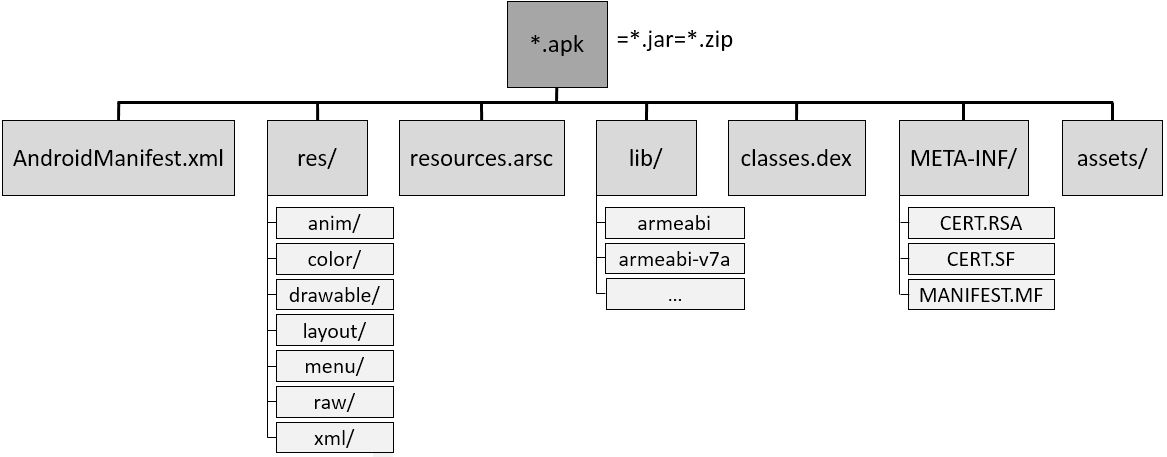
\includegraphics[width=\textwidth]{figures/apk_content}
  \caption[APK Content]{Contents of the APK file}
  \label{fig:apk_content}
\end{figure}

The \code{AndroidManifest.xml} file holds metadata information
about the app like the package name, it's version, a list of
activities and required permissions. \code{resources.arsc}
does contain precompiled resources like strings, styles
or binary XML. Developers can use the \code{assets/} folder
to store raw data needed for the app like music files,
fonts and so on. If the app does make use of the JNI,
the \code{lib/} folder does contain compiled library directories
for every supported CPU architecture (armeabi, x86, \ldots).
Every resource which is directly addressed from Android code
is stored in the \code{res/} folder including xml files for
layouts and menus. The \code{META-INF/} directory does hold
the signatures for the specific app similar to a JAR file.
The heart of every app is the \code{classes.dex} that does
contain the application code in form of the DEX format
specified by Google ~\parencite{dex}. The Java Development
Kit (JDK) tool ``javac'' creates a JAR out of every inputted
 \code{.java} file. The Google build tool ``dx'' takes over
 the transition from \code{.jar} to \code{.dex} ~\parencite{dxtool}.

\section{App installation process}\label{section:app_installation}
As in \autoref{section:android_apps} described, apps are distributed
in form of APK files. This chapter describes what happens next to
the APK file.

The APK file gets forwarded to the Android ``Package Manager''(pm)
which then calls the \code{installPackage()} method for this
APK. Among other things, the pm copies the original \code{*.apk}
to the path \code{/data/app/<package>.<appname>-1/base.apk}.
The \code{lib/} directory is getting extracted and gets also copied
into that path. \code{classes.dex} gets optimized by either ``dexopt''
or ``dex2oat'' depending which runtime is present (DVM or ART).
The outcoming file is in both cases no more device independent
and lies at \code{/data/dalvik-cache/<arch>/} with the name
\code{data@app@<packagename>.<appname>-1@base.apk@classes.dex}.
It does represent the last stored unit of an app that gets
executed. Attention should be paid to the file extension.
It's the same with both runtimes but is actually a totally
different file format.
Therefore the name of the file is just a reference to the path
of its source when replacing the ``@'' characters with ``/''.
If the present runtime is DVM thus Android < 5.0, the generated
file format is ODEX (Optimized DEX) and otherwise
ELF 32/64 (Executable Linking Format) although the responsible
tool for that conversion step is called ``dex2oat''. This ELF
file also gets analyzed in the course of this thesis
(it does however hold an ``OAT'' file among other things so that
the tool name actually does makes sense).
To give an app the possibility to
store some data, a \code{/data/data/<appname>} directory is
also created.

Last but not least, the pm adds entries to the
\code{/data/system/packages.xml} as well as the
\code{/data/system/packages.list} files. They do contain
meta information about the installed packages like
required permissions and the UID/GID of that instance.
Android uses that UID/GID to enforce the sandboxing model
~\parencite{securityinternals}.
\autoref{fig:app_installation} shows the explained
relevant actions the pm performs.

\begin{figure}[htb]
  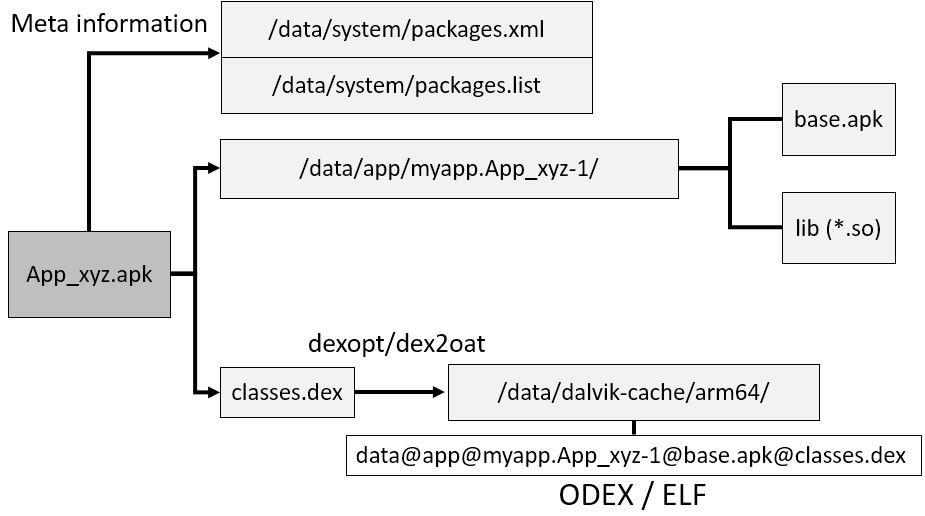
\includegraphics[width=\textwidth]{figures/app_installation}
  \caption[App installation process]{App installation process}
  \label{fig:app_installation}
\end{figure}

\section{App execution process}
